\chapter{Objectives} % Function and Non-Functional requirements

In order to ensure our system fulfils its intended purpose, we have devised a formal list of requirements. This will allow us to track progress and measure the success of the project. The requirements have been categorised and prioritised, according to the MoSCoW method. In particular, ``must'' means that a requirement is essential for the project and will be considered first. ``Should'' denotes the requirements that are important but not strictly necessary. ``Could'' means that a requirement is of less importance and will be implemented provided that the time constraints allow it. We have also identified the objectives which are out of scope for this project, and therefore will not be implemented. Such objectives are labelled as ``won't''.

\section{Objective List}
% Feel free to add/change anything
\begin{enumerate}
    \item Problem domain
    \begin{enumerate}
        \item The system \textbf{must} facilitate writing code for common SPH problems.
        \item The system \textbf{won't} support other problems outside of the SPH domain, such as gravitational interaction or Discrete Vortex Method (DVM).
    \end{enumerate}
    \item Input code
    \begin{enumerate}
        \item The system \textbf{must} handle input code written in C++, potentially with some syntax extensions.
        \item The system \textbf{should} use existing C++ syntax whenever possible.
        \item The system \textbf{could} process written equations into kernel functions for the user.
        \item The system \textbf{won't} process input code written in other languages, such as Python.
    \end{enumerate}
    \item API design
    \begin{enumerate}
        \item The system \textbf{must} expose a low-level API, similar to OPS and OP2.
        \item The system \textbf{should} allow the user to implement some functions in a platform-specific way (e.g. if they want to integrate an existing SPH HPC library).
        \item The system \textbf{could} implement a high-level API, to further simplify developing SPH simulations (e.g. use operator overloading to allow the user to define parts of the program as equations).
    \end{enumerate}
    \item Target platforms
    \begin{enumerate}
        \item The system \textbf{should} support multiple target processor architectures.
        \item The system \textbf{should} be able to generate code for OpenMP.
        \item The system \textbf{should} be able to generate code for CUDA.
        \item The system \textbf{could} be able to generate code for MPI.
        \item The system \textbf{could} implement combinations of platforms, such as CUDA + OpenMP or CUDA + MPI.
    \end{enumerate}
    \item Performance
    \begin{enumerate}
        \item The system \textbf{should} generate code that achieves performance no more than 10\% slower than the reference miniapp implementations.
        \item The system \textbf{could} implement more advanced optimisations to further improve performance.
        \item The system \textbf{should} be able to compile input code in reasonable time.
    \end{enumerate}
\end{enumerate}

\section{System Overview}

Figure \ref{fig:arch-diagram} gives a broad overview of the proposed project architecture to meet the above objectives. Broadly, we take the C++ code written with our DSL, and parse it. Extract the AST and then generate suitable code for one of a number (or a combination) of backend hardware using a template engine. In the process, applying transformations or optimisations as necessary. This is then compiled by the usual C++ toolchain, which can apply further compiler optimisations. Optionally, if time permits, we want to also develop a separate parser which can take a more elementary equation based representation of the SPH simulation and convert that into a representation based in our DSL.

\begin{figure}[H]
    \centering
    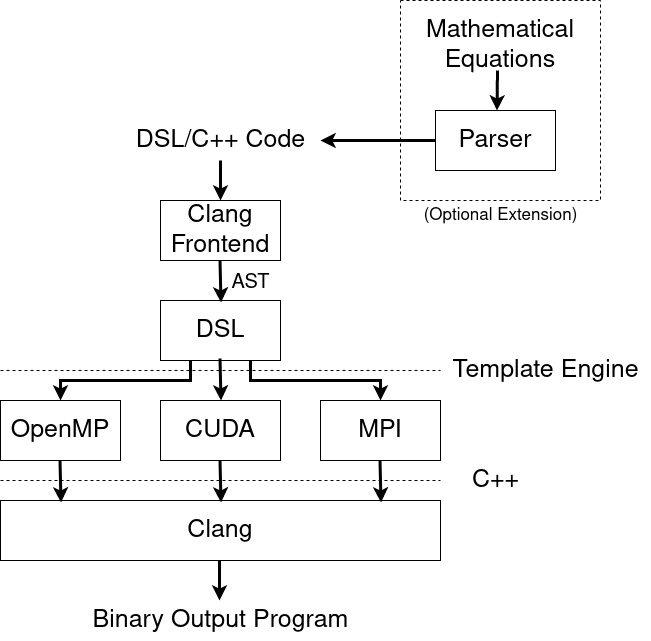
\includegraphics[width=0.8\textwidth]{thesis/diagrams/architecture.jpg}
    \caption{Overview of the proposed project architecture.}
    \label{fig:arch-diagram}
\end{figure}